\documentclass{standalone}
\usepackage{tikz}
\usetikzlibrary{shapes.geometric, arrows, positioning}

\begin{document}

% ============================================================
% 1. HYBRID ML + DL + ANOMALY ARCHITECTURE
% ============================================================
\begin{tikzpicture}[node distance=2cm, auto]
    \node [rectangle, draw, rounded corners] (input) {Input Data};
    \node [rectangle, draw, rounded corners, right=of input] (ml) {ML Models\\RF, SVM, GBM};
    \node [rectangle, draw, rounded corners, right=of ml] (dl) {Deep Learning\\Autoencoder};
    \node [rectangle, draw, rounded corners, right=of dl] (anomaly) {Anomaly Models\\IF, OC-SVM};
    \node [rectangle, draw, rounded corners, right=of anomaly] (fusion) {Hybrid Fusion};
    \node [rectangle, draw, rounded corners, right=of fusion] (output) {Detection Result};

    \draw[->] (input) -- (ml);
    \draw[->] (ml) -- (dl);
    \draw[->] (dl) -- (anomaly);
    \draw[->] (anomaly) -- (fusion);
    \draw[->] (fusion) -- (output);
\end{tikzpicture}

\vspace{2cm}

% ============================================================
% 2. AUTOENCODER DIAGRAM
% ============================================================
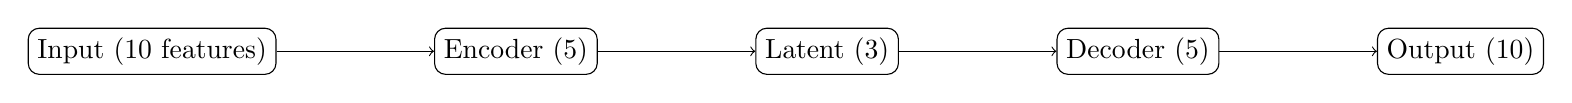
\begin{tikzpicture}[node distance=2cm, auto]
    \node [rectangle, draw, rounded corners] (input) {Input (10 features)};
    \node [rectangle, draw, rounded corners, right=of input] (enc) {Encoder (5)};
    \node [rectangle, draw, rounded corners, right=of enc] (bottleneck) {Latent (3)};
    \node [rectangle, draw, rounded corners, right=of bottleneck] (dec) {Decoder (5)};
    \node [rectangle, draw, rounded corners, right=of dec] (output) {Output (10)};

    \draw[->] (input) -- (enc);
    \draw[->] (enc) -- (bottleneck);
    \draw[->] (bottleneck) -- (dec);
    \draw[->] (dec) -- (output);
\end{tikzpicture}

\vspace{2cm}

% ============================================================
% 3. ISOLATION FOREST LOGIC
% ============================================================
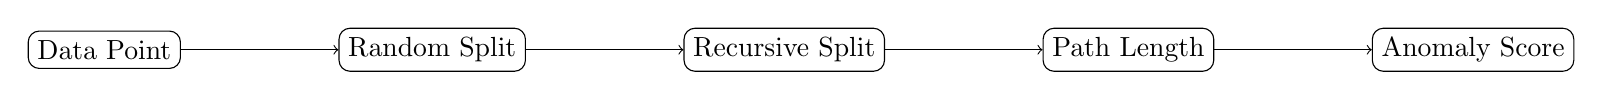
\begin{tikzpicture}[node distance=2cm, auto]
    \node [rectangle, draw, rounded corners] (start) {Data Point};
    \node [rectangle, draw, rounded corners, right=of start] (split1) {Random Split};
    \node [rectangle, draw, rounded corners, right=of split1] (split2) {Recursive Split};
    \node [rectangle, draw, rounded corners, right=of split2] (path) {Path Length};
    \node [rectangle, draw, rounded corners, right=of path] (score) {Anomaly Score};

    \draw[->] (start) -- (split1);
    \draw[->] (split1) -- (split2);
    \draw[->] (split2) -- (path);
    \draw[->] (path) -- (score);
\end{tikzpicture}

\end{document}
